\setcounter{page}{1}

\chapter{Lightning Network}

\newcommand{\noteOnBitcoinNaming}[0]{
    \footnote{
        From now till the end of the document we will use the word Bitcoin Protocol and
        Bitcoin with capitalized to identify the protocol, and the word bitcoin not capitalized to identify the currency
    }
}

\newcommand{\noteOnCLNImpl}[0]{
    \footnote{
    core lightning is one of the main implementations today, and it is available at
    \href{https://github.com/ElementsProject/lightning}{https://github.com/ElementsProject/lightning}
    }
}



\section{Introduction}

The \emph{Lightning Network} is a peer-to-peer protocol that proposes a scalable solution for Bitcoin\noteOnBitcoinNaming where one
of the goal of the proposal is to be able to execute micro-transaction with it.
In fact, Bitcoin does not scale for a sequence of reasons, and one of them is the number of
maximum rate transactions that the network can process.\\
Therefore, with the awareness that some of these limitations that are feature in Bitcoin, the lightning network try to solve
the scalability problem by offering an \emph{off-chain} solution that enables peers to exchange partially
signed transaction without violating the Bitcoin rules.\\
Lightning Network is proposed for the first time in the 2015 in a draft paper \cite{lightning-network-paper},
and then implemented in the 2018 with the \emph{c-lightning}\noteOnCLNImpl (aka \emph{core lightning}) implementation.
However, the protocol is evolving over the years by a process of standardization\cite{lightning-bolts}, and the paper is considered
only a written idea on how to build an off-chain solution without any definition of the current protocol state machine.

\section{Off-Chain Protocol}

The Bitcoin network has scalability problems in confront of the modern payment system that people use daily.
In particular, these problems are related to the space required by the blockchain to store each transaction,
and the relatively long time that is required to consider a transaction confirmed in the blockchain.

In fact, the payment network Visa achieved around 65,000\cite{visa-sheet} transactions per second, and currently,
Bitcoin supports around 7 transactions per second with a required space estimated of 1 megabyte per block. Considering,
an average of 300 bytes per bitcoin transaction and assumed unlimited block sizes, the space for storing the same number
of transactions is estimated in the order of terabytes\cite{lightning-network-paper}.

Therefore, in order to use the Bitcoin protocol as an alternative of the current system for a subset of
the problem, such as the accessibility to the modern world to people that live in not developed places (e.g Africa),
there is a need to scale the protocol.

This kind of problem is almost considered a well studied problem, and different solutions are given in different
way, that most of the time required a hard fork (See Section \ref{sec:hard_vs_soft} for the definition of hard fork) of the protocol itself.
One of the most popular hard fork examples is given by Bitcoin Cash which increases the block size to be able to insert
inside a block more transactions.
However, in the Bitcoin ecosystem (based on the Bitcoin Core implementation) the idea of a hard fork is considered an
end of choice alternative and some of the ideas to solve the scalability of the protocol are proposed through Bitcoin Script trick
that sometimes required a soft fork in the base protocol itself.

\section{Lightning Network Basics}

The actual Lightning Network is more complicated than what was described in \cite{lightning-network-paper}, and it is
evolved a lot from the first time that the paper came out. However, the idea described in the paper was an evolution
of some previous ideas regarding the possibility to have payment channels with Bitcoin.

\subsection{Payment Channel}

A Payment Channel also known as Micropayment Channel is class of techniques designed to allow users to make multiple
Bitcoin transactions without committing all of the transactions to the Bitcoin blockchain. In a typical payment channel,
only two transactions are added to the blockchain but an unlimited or nearly unlimited number of payments
can be made between the participants.\\
In fact, the concept of replacing an old transaction with the new one is proposed from \emph{Satoshi Nakamoto}\footnote{TODO: described who this guy is} in the mainlist\cite{payment-channels-satoshi}, and
the basic concept to implement this feature was present from the version 0.0.1 of Bitcoin core. However, this solution
was not completely safe because with this method there is the possibility to steal funds from the other party or parties.\\

Later, there is a new proposal to implement this kind of concept called \emph{Spillman-style payment channels}, and it is
implemented inside a \emph{bitcoinj}\cite{bitcoinj-impl}. Spillman payment channels are unidirectional where
there is a payer and a payee, in this kind of channel it is not possible to transfer money back in the reverse direction, and the payment
channels expire after a specific time.
In addition, the receiver needs to close the channel before the expiration time.
However, this proposal has malleability problems solved later by the \emph{BIP  65}\cite{bip65} Bitcoin proposal that includes a new Bitcoin Script OP code
called \emph{OP\_CHECKLOCKTIMEVERIFY} that unlock a new version of the \emph{Spillman-style payment channels}.\\
While the idea of payment channels start to be explored around the Bitcoin community, two new proposals came out that are
\emph{Poon-Dryja payment channels}\cite{lightning-network-paper} (currently used in the Lightning Network),
and \emph{Decker-Wattenhofer duplex payment channels}\cite{Decker2015fast} where these proposals try to improve the known state
of the art by allowing more complex payment channel operations.

In particular, the Poon-Dryja payment channel is proposed in \cite{lightning-network-paper}, where
the funds are locked into a 2-of-2 multisig\footnote{TODO: cite a definition maybe in my betchelor},
but before the funding transaction is even signed, commitment transactions for each party are first written and signed.\\
Therefore, these operation requires referring to transactions that have not been signed yet, and this requires to use a transaction
the format that separates signatures from the part of the transaction that is hashed to generate the txid, such as Segregated Witness.\\
One of the proprieties proposed by the Poon-Dryja payment channel is how the channels can be closed:

\begin{itemize}
  \item Unilateral close: to close a channel required only that one side is involved. This is useful when one
        of the party start to be unresponsive, and when this happens, the funds of
        the party that closed the channel is temporarily time-locked, and this leaves the opportunity to
        track the special on-chain transaction on the blockchain;
  \item Bilateral close: to close a channel the two-party cooperate, and when this happens the result
        on-chain transaction looks like a normal 2-2 multisig transaction.
\end{itemize}

On the other hand, the Decker-Wattenhofer duplex payment channel proposal came out at the same time as the previous proposal, and
it requires a new \emph{BIP 68}\cite{bip68} proposal that enforce a more strictly semantics on \emph{nSequence}, and the propose is to
establish two unidirectional Spillman payment channels in both
direction, where these channels referees to the nSequence instead of the nLockTime.\\
However, instead of funding unidirectional payment channels directly from an on-chain funding transaction, there is an \quotes{invalidation tree} of off-chain transactions between the funding transaction and the payment channel finalization transactions.

\section{Lightning Network implementation}

The basic idea of the Lightning Network proposed in \cite{lightning-network-paper} is based on using Bitcoin Script
to allow the possibility to exchange not final transaction between participants as Figure \ref{fig:ln-onchain} shows.
However, the actual Lightning Network implements a tech stack that looks more complicated (Figure \ref{fig:lightning-stack}).\\
In fact, the Lightning Network implements a new \emph{Peer to Peer} protocol that exchanges information through
a gossip protocol. For this reason, the state machine of the Lightning Network
can be very complicated in some specific cases.

\begin{figure}[h]
  \begin{center}
  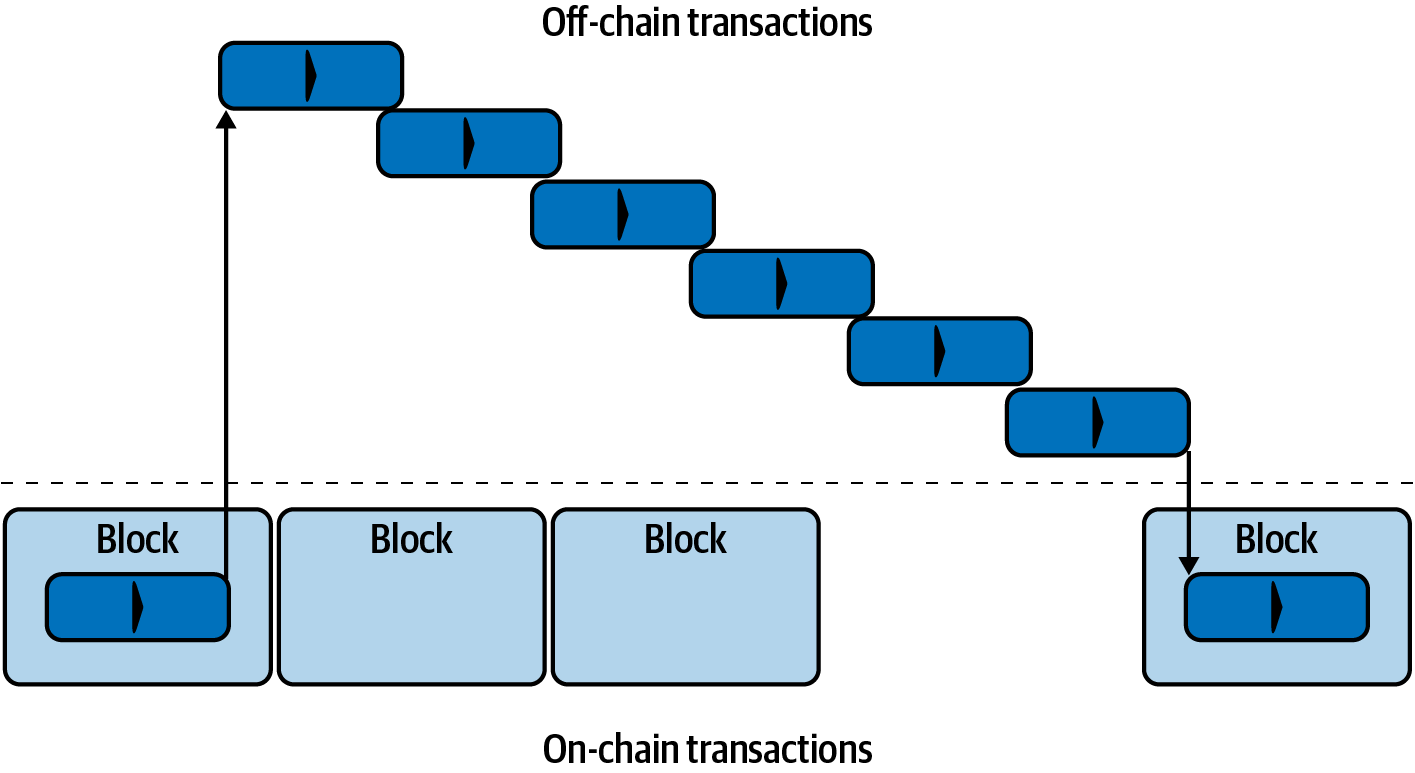
\includegraphics[width=0.6\columnwidth]{imgs/mtln_0702.png}
  \end{center}
  \caption{Diagram provides an overview of how the open and close a channel operations work.}
  \label{fig:ln-onchain}
\end{figure}


\begin{figure}[h]
  \begin{center}
  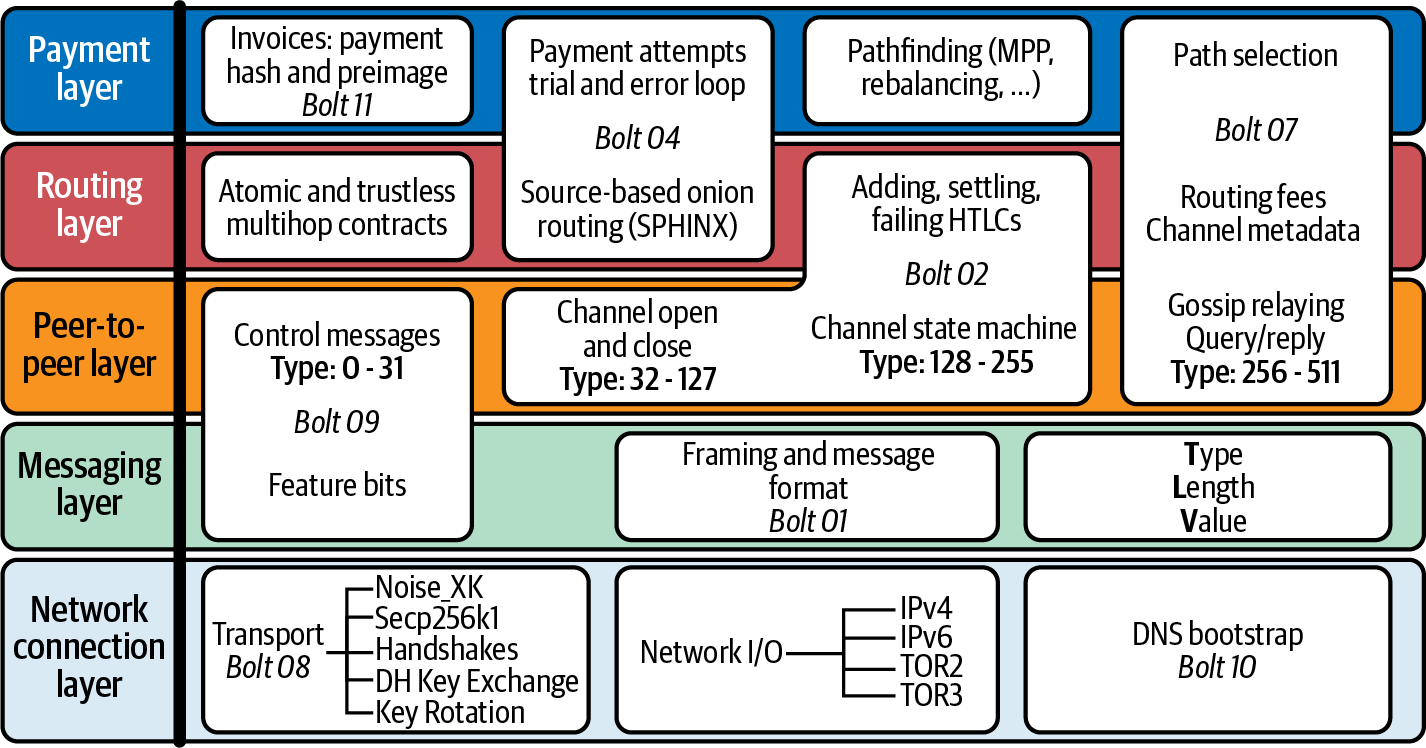
\includegraphics[width=0.6\columnwidth]{imgs/mtln_0601.png}
  \end{center}
  \caption{Diagram provides an overview of these layers and their component protocols.}
  \label{fig:lightning-stack}
\end{figure}

The following Section there is described a general overview of how the Lightning Network is implemented through the
\emph{BOLT} specification\footnote{BOLT: Basis of Lightning Technology (Lightning Network Specifications)}.

\subsection{Lightning Network Specifications}

Since 2017 the lightning network start to be implemented by different entities,
and due the high overview of the Lightning Network state machine definition in \cite{lightning-network-paper}
the implementations start to cooperate in a Specification that all the lightning implementations agree on.

Therefore, the specification describes the following concept to allow full interoperability between implementations:

\begin{itemize}
  \item BOLT 1: describe the basics of the protocol, like how a message is encoded and what type of messages are required in order to support the communication;
  \item BOLT 2: describe the peer-to-peer protocol for channels managements. This is one of the core concepts of lightning, in fact after a payment channel
        is settled up, the channels can have different cases that are described in the Section \ref{sec:channel_state}
  \item BOLT 3: describe how the Bitcoin script language is used to compose the
        payment channel, and what kind of Bitcoin transactions are involved.
  \item BOLT 4: describe the onion routing protocol that it is used to exchange messages between peers which in this case are called \emph{hop}.
        The routing schema is based on the \emph{Sphinx}\cite{sphinx} construction and is extended with a per-hop payload.
  \item BOLT 5: describe how the on-chain transaction should be handled.
  \item BOLT 7: describe how the peer-to-peer node and channels are discovered through the network;
  \item BOLT 8: describe all the authenticated and encrypted transport protocols;
  \item BOLT 9: describe how the feature flags\footnote{Feature flags that are used to establish what kind of feature are supported by a node} need to be managed;
  \item BOLT 10: describe the DNS Bootstrap and Assisted Node Location;
  \item BOLT 11: describe the invoice protocol for the lightning network protocol;
\end{itemize}

To add a new feature inside the protocol it needs to be discussed between implementations and when at least two implementations supports the feature, it is considered standard.\\
The actual implementations that are compliant and contribute to the lightning network specification are:

\begin{itemize}
  \item \emph{core lightning}: it is the first implementation written in C, and it is written
        to be an efficient solution for servers. In addition, it is focused on improving the lightning network specification. In fact, core lightning has several new proposals like the \emph{BOLT 12}\footnote{BOLT 12 is a new proposal to perform
        lightning payment and improve several problems that exists in the BOLT 11.} implemented and in discussion to be
        added inside the standard protocol;
  \item \emph{lnd}: a lightning network implementation written in Go lang. It is one of the most used lightning network implementations in according to \footnote{add the topology paper there};
  \item \emph{ldk}: a lightning network implementation written in rust, that provides the lightning building blocks exposed as Library;
  \item \emph{eclair}: a lightning network implementation written in Scala, widely used on mobile wallets, but it is written to
        support server side too.
\end{itemize}

\section{Lightning Network Channel Operation}
\label{sec:channel_state}

The channel state management defines the state machine of the channels, and they are described in the BOLT 2 specification. Currently, it is a very complex
state machine where there are involved several steps in order to avoid bad
situations where a node can steal funds or lock the funds involved in the blockchain for a long period.\\
In this section will be introduced a deep introduction to the primary operations to create and manage channels.

\subsection{Channel Establishment}
\label{sec:open_a_channels}

Opening a channel between two peers involves several steps before arriving at the point to construct the Bitcoin transaction also
known as \emph{funding transaction}.
In fact, the Lightning Network protocol requires some connection steps between the two peers start to open a channel, this
operation is defined inside the BOLT 2\cite{bolt2} as \emph{Channel Establishment}.

For this reason, each public peer is exposes to one or more public IP addresses where
they are listening for incoming connections, and when a peer wants to open
a channel with a specific peer the following information must be provided:

\begin{itemize}
  \item Node ID: It is the node's public key, differently from Bitcoin in this case it is public and it is one of the information included inside the gossip by the node;
  \item Node IP address and port: Where the node it is listening for an incoming connection.
\end{itemize}

In addition, most of the node support also the Tor network, but with the current usage of the protocol the Tor network provides very unreliable
performance as discussed in the Section \ref{sec:payment_forwarding}.\\
After the node is connected with the counterpart, the Channel Establishment can be performed, and a sequence
of messages is exchanged (Figure \ref{fig:channel-establishment}). During this process
the following protocol messages are involved:

\begin{itemize}
  \item {\bf open\_channel}: The node that wants to open a channel (sender) creates an open channel message where the information of the
        Blockchain Network are defined (It is not required that this network need to be the Bitcoin network);
  \item {\bf accept\_channel}: The node that receives the open channel request (receiver) with the information of the Blockchain network to use
        can accept the request to open a channel by sending an accept channel message that contains the Blockchain network information, and
        a \emph{temporary\_channel\_id} generate from the peer information.
  \item {\bf funding\_created}: The sender after receiving the confirmation that the counterpart is ready to open a channel
        send a funding created message with the initial information of the funding transaction created as described in the Section \ref{sec:lightning_network_contract}
  \item {\bf funding\_signed}: After the sender communicate the initial information for the funding transaction, the
        the receiver can send the signature for the funding transaction through a funding signed message, and at this moment the temporarily
        channel id sent in the previous steps can be overridden by a real channel id generated from the on-chain transaction information.
  \item {\bf funding\_lock}: The sender after committing the transaction on-chain can send a message funding lock to the counterpart when
        the on-chain transaction has reached enough confirmation. This message is also know as \emph{channel\_ready} message in the BOLT 2\cite{bolt2}.
\end{itemize}

\begin{figure}[h]
  \begin{center}
  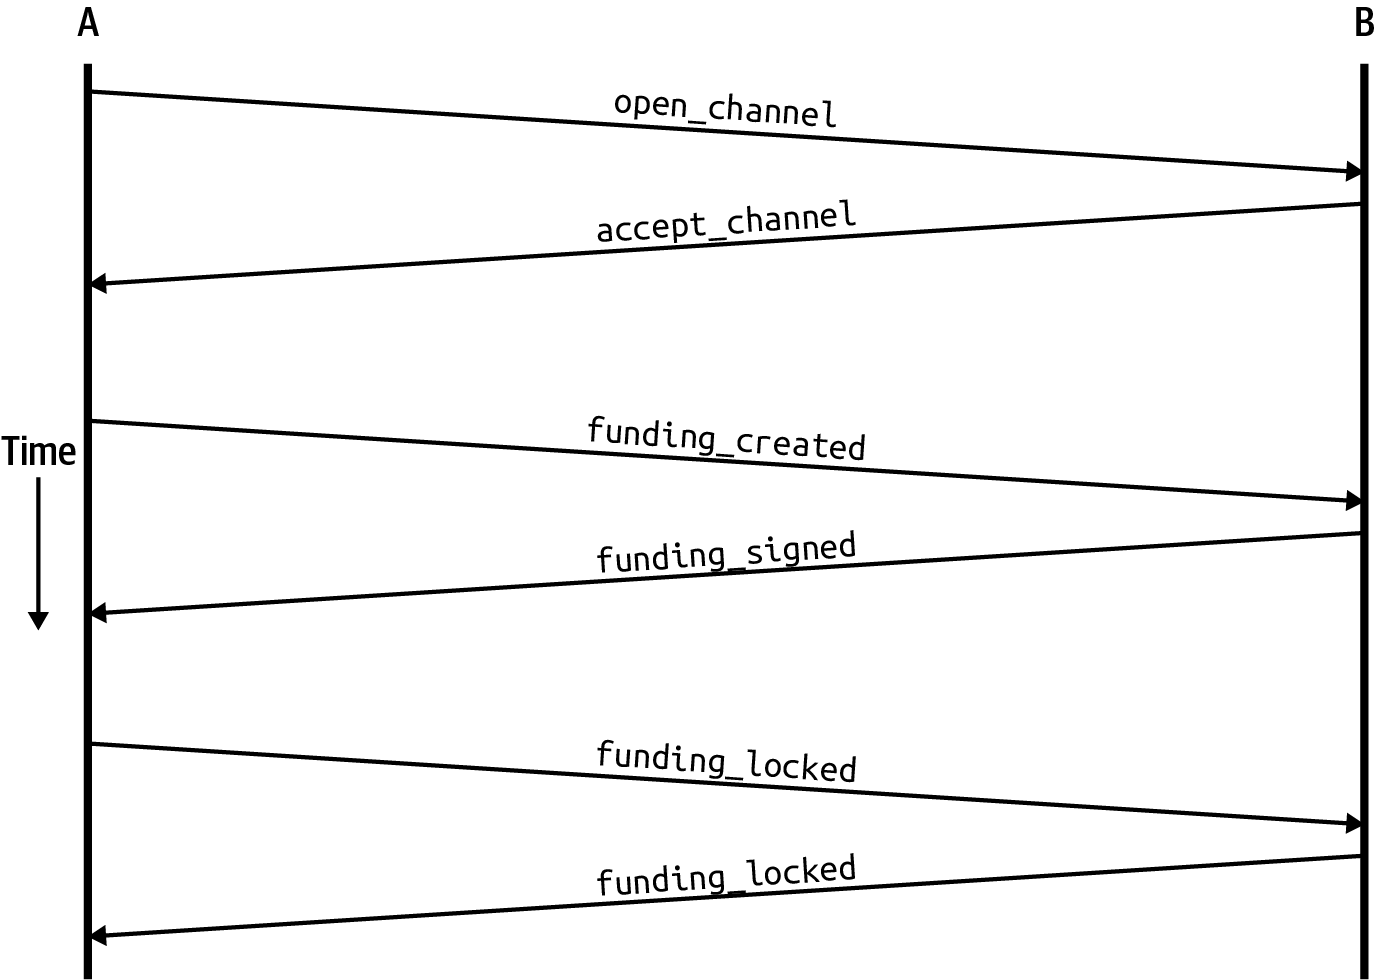
\includegraphics[width=0.6\columnwidth]{imgs/mtln_0703.png}
  \end{center}
  \caption{Channel Establishment procedure workflow.}
  \label{fig:channel-establishment}
\end{figure}

After the funding transaction is confirmed on the blockchain and the channel is ready to be used (this state of the channel is also know as \emph{normal state}),
peers can perform lightning payments that can modify the state of the current channel, in the Section \ref{sec:modify_channel_state} is described how
these operation are performed inside the protocol.

\subsection{Modify Lightning Channel State}
\label{sec:modify_channel_state}

The Lightning network protocol complexity with the current implementation (defined in \cite{lightning-bolts})
is generate from the channel state management that need to ensure that there are no situation that can
cause  possibilities to lost funds from one participant.\\
In fact, if one peer has an outdated channel state, and this state is shared with the network, the counterpart can
detect this inconsistency between the real channel state and the one received. In this case, the peer can and must
perform the punishment operation that the lightning network define in \cite{bolt2}, where the channel between the two peers
is closed and the the receiver of the outdated channel state take all the currency involved.\\
However, this operation of punishment can also be performed on peers that has bug in the software and publish an old state of the
channel due a corrupted database. In this case propose like \cite{eltoo} described in the Section \ref{sec:eltoo} offers
better solutions for channel state management.

\subsubsection{Forwarding Lightning Payments}

The Lightning Network protocol allow payments through the network by sending an partial sign transaction that
allow peers to perform payment in the network.
Therefore, in order to perform a payment the state the channel need to be alterate, and in some case the payment can involve
different peers long a \emph{route path}.\\

\section{Lightning Network Payments Forwards}
\label{sec:payment_forwarding}

Describe how the payment are forwarded

\section{Lightning Network Extension}
\label{sec:eltoo}

Describe Eltoo\cite{eltoo} payment channels.
